\documentclass{beamer}




\usepackage[T1,T2A]{fontenc}
\usepackage[utf8]{inputenc}

\usepackage{graphicx}
\usepackage{blindtext}
\usepackage{ mathrsfs }
\usepackage[russian,english]{babel}
%\usepackage{ dsfont }

\author{Деркач Максим Юрьевич}
\title{Криптографические протоколы}
\subtitle{Протоколы WEP, WPA, WPA2, WPA3}
\setbeamercolor{frametitle}{bg=cyan!10}


%\usetheme{lucid}
\begin{document}
	\frame {
		\titlepage
	}
	\frame {
		\frametitle{Ссылки}
		
		\url{https://www.cs.jhu.edu/~Eastubble/dss/ae.pdf}
		\url{http://cseweb.ucsd.edu/~mihir/papers/oem.pdf}
		\url{https://habr.com/en/post/425637/}
				
			
	}
	\frame{
		\frametitle{Введение}
		\textbf{WEP (Wired Equivalent Privacy)} - один из старейших протоколов безопасности, который может использовать WiFi-маршрутизатор, и он не очень безопасный. Он был использован в 1990-х годах, но с тех пор были разработаны другие протоколы безопасности.
		
		\textbf{WPA (Wi-Fi Protected Access)} - это протокол, который первоначально заменило WEP как более безопасный способ хранения данных. В то время он был не идеален, но он лучше, чем WEP. Весь смысл разработки этого протокола состоял в том, чтобы преодолеть некоторые из основных недостатков WEP.
	}

	\frame{
	\frametitle{WEP}

В основе WEP лежит поточный шифр \textbf{RC4}, выбранный из-за своей высокой скорости работы и возможности использования переменной длины ключа. Для подсчета контрольных сумм используется \textbf{CRC32}. 

\bigskip


}

\bigskip
	\frame{
	\frametitle{WEP}
	
	Пакет WEP протокола состоит из 2 частей:
	\begin{enumerate}
		\item Открытые данные:
		\begin{enumerate}
			\item Синхропосылка (IV) - 3 байта;
			\item Пустое место (Padding) - 6 бит;
			\item Идентификатор ключа (Key ID) - 2 бит;
		\end{enumerate}
		\item Зашифрованные данные:
		\begin{enumerate}
			\item Данные
			\item Контрольная сумма
		\end{enumerate}
	\end{enumerate}
	
	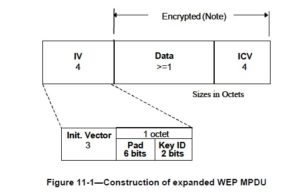
\includegraphics[width=0.8\linewidth]{wep_packet.jpg}
}

	\frame{
	\frametitle{WEP Auth Protocol}
		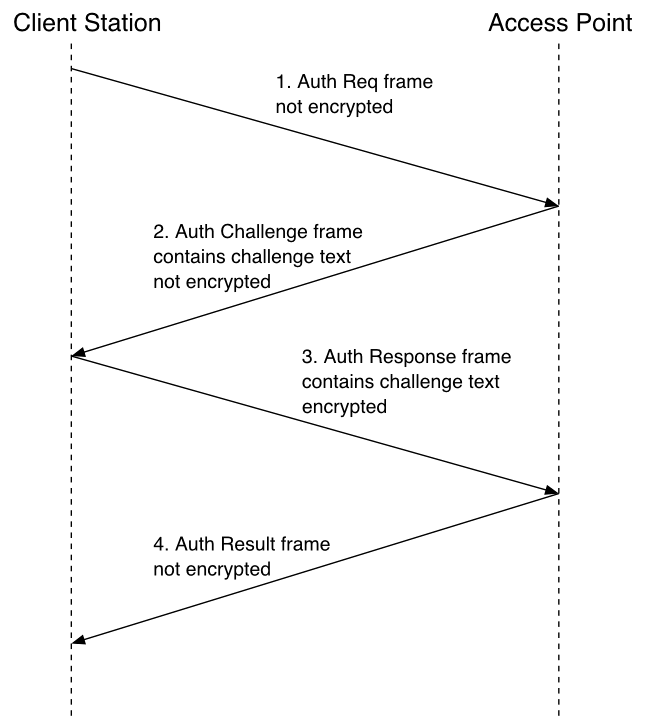
\includegraphics[width=0.7\linewidth]{wep_protocol.png}
}

\frame{
	\frametitle{WEP Encryption and Decryption}
		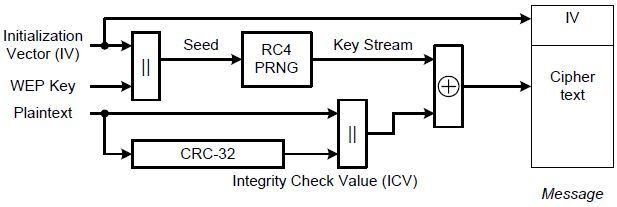
\includegraphics[width=0.8\linewidth]{wep_encap.png}
		
		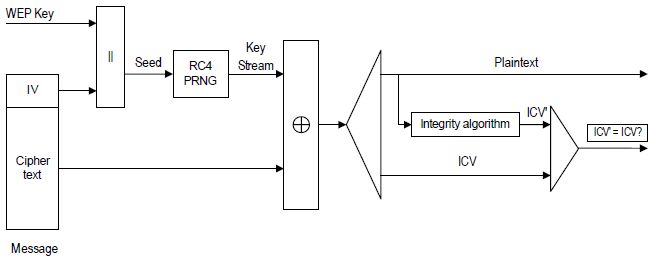
\includegraphics[width=0.8\linewidth]{wep_decap.png}
}

\frame{
	\frametitle{WEP Keys}
		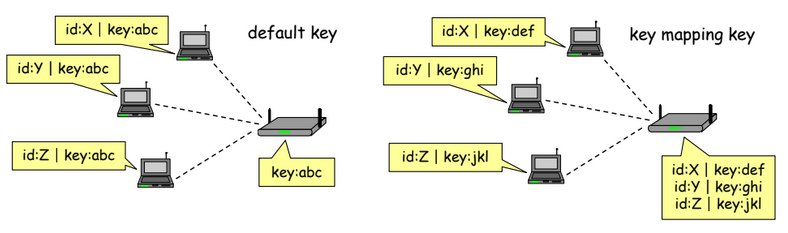
\includegraphics[width=0.8\linewidth]{wep_keys.jpg}
}

\frame{
	\frametitle{WEP Security}
	В протоколе WEP есть множество слабых мест:
	\begin{enumerate}
		\item Механизмы обмена ключами и проверки целостности данных:
		\begin{itemize}
		\item В качестве MAC функции в WEP используется некриптографический алгоритм CRC.
		\end{itemize}	
		\item малая разрядность ключа и вектора инициализации:
		\begin{itemize}
		\item Повторное использование IV создает идентичные ключевые потоки, и поскольку длина IV мала, это гарантирует, что IV повторится через относительно короткое время (5-7 часов) в загруженной сети.
		\item Стандарт 802.11 не описывал ограничения и правила на генерацию IV. Поэтому некоторые производители беспроводных адаптеров генерировали одинаковые последовательности IV, постоянное IV. В результате хакеры могли записывать сетевой трафик, определять поток ключей и использовать его для расшифровки зашифрованного текста.
	\end{itemize}
\end{enumerate}
}
\frame{
	\frametitle{WEP Security}
	
\begin{enumerate}
\item Способ аутентификации:
\begin{itemize}
\item Одностороняя аутентификация, $AP$ - не аутентифициорован.
\item В результате аутентификация не устанавливается сессионный ключ.
\end{itemize}
\item Алгоритм шифрования.
\end{enumerate}

\bigskip
\textbf{Authentication}
\begin{enumerate}
\item ...
\item $AP->STA:r$
\item $STA->AP:IV|r \oplus K$
\item ...
\end{enumerate}

\bigskip
Атака
\begin{enumerate}
	\item ...
	\item $AP->I(STA):r'$
	\item $I(STA)->AP:IV|r'\oplus K$
	\item ...
\end{enumerate}
}

\frame{
	\frametitle{WEP Security}
	\textbf{CRC}:\\
	
	$CRC(X \oplus Y) = CRC(X) \oplus CRC(Y)$
	
	\bigskip
	
	\textbf{Атака}\\
	
	$((M | CRC(M)) \oplus K) \oplus (\hat{M} | CRC(\hat{M}) = $ \\
	$((M \oplus \hat{M}) | (CRC(M) \oplus CRC(\hat{M})) \oplus K$
}

\frame{
	\frametitle{WPA | 802.11i}
	Улучшения в 802.11i:
	\begin{enumerate}
		\item Добавлен фраймворк аутентификации(EAP).
		\item Алгоритмы шифрования и целостности испозьуют разные ключи.
		\item Улучшенна защита целостности.
		\item Улучшенна защита конфиденциальности.
	\end{enumerate}

	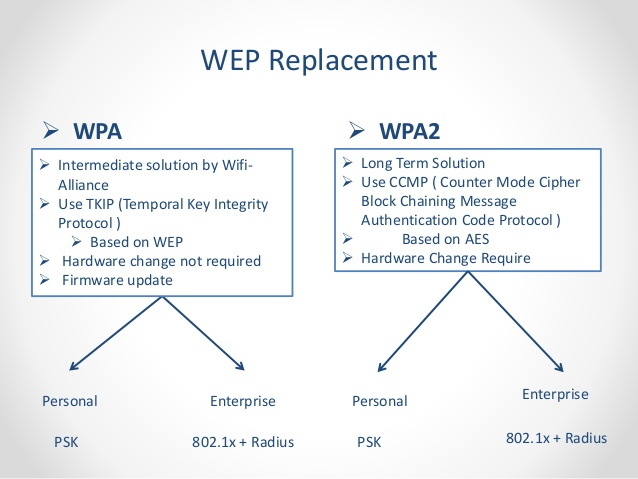
\includegraphics[width=0.6\linewidth]{wfi_table3.jpeg}
}

\frame{
	\frametitle{WPA-PSK}
	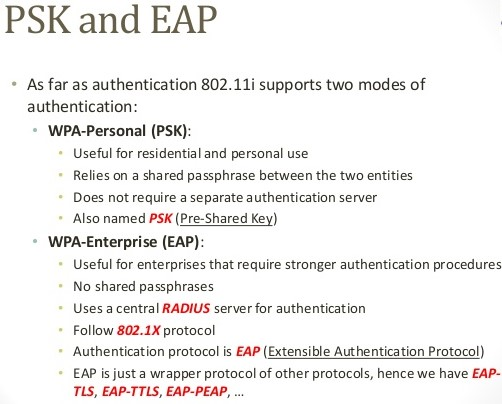
\includegraphics[width=0.8\linewidth]{wpa_types.jpeg}
}


\frame{
	\frametitle{WPA Структура ключей}

	Начальный процесс аутентификации выполняется либо с использованием предварительного общего ключа pre-shared key (PSK), либо после обмена EAP через 802.1X. \\
	
	\bigskip
	
	Этот процесс гарантирует, что клиентская станция (STA) аутентифицирована с точкой доступа (AP). \\
	
	\bigskip
	После аутентификации PSK или 802.1X генерируется общий секретный ключ, называемый \textbf{ парным главным ключом Pairwise Master Key (PMK) }. \\
}

\frame{
	\frametitle{WPA Структура ключей}
\textbf{Групповой временный ключ (GTK)}, используемый в сети, может нуждаться в обновлении из-за истечения предварительно установленного таймера. Когда устройство покидает сеть, GTK также необходимо обновить. Это сделано для того, чтобы устройство не получало больше многоадресных или широковещательных сообщений от точки доступа.

\bigskip
Для обновления группового ключа, происходит 2-этапное рукопожатие:

\bigskip
\begin{enumerate}
	\item $AP->STA: E_{KEK}(\hat{GTK})|T|MIC_{KIK}$
	\item $STA->AP: T+1|MIC_{KIK}$
\end{enumerate}

}

\frame{
	\frametitle{WPA Структура ключей}
	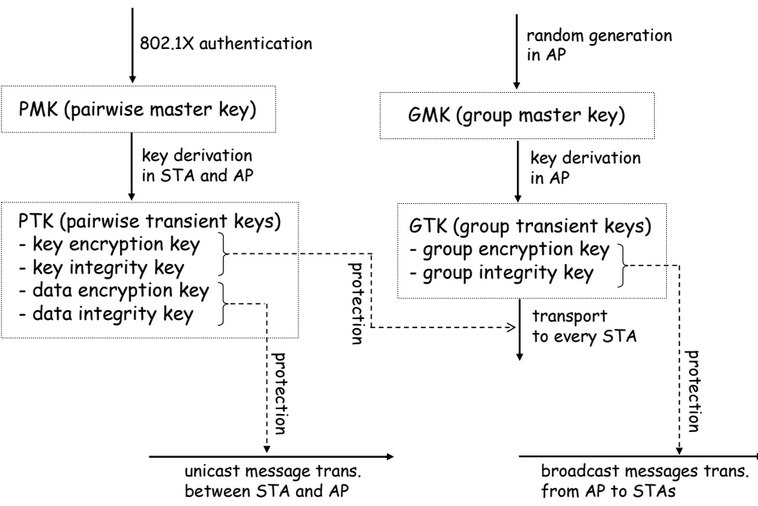
\includegraphics[width=0.9\linewidth]{wpa_keys.jpg}
}


\frame{
	\frametitle{WPA Структура ключей}
	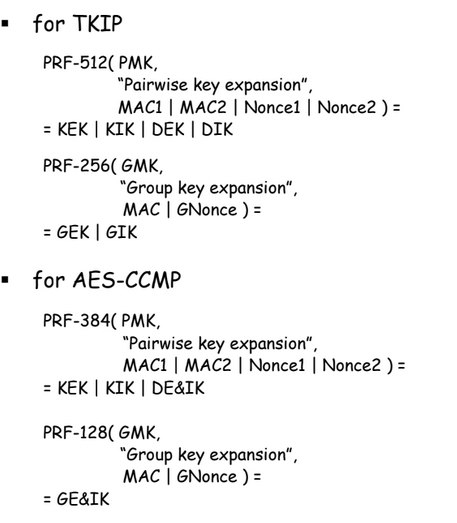
\includegraphics[width=0.7\linewidth]{wpa_key_gen.jpg}
}

\frame{
	\frametitle{Протокол аутентификации (Four-way handshake)}
	\textbf{Задачи}:
	\begin{enumerate}
	\item Доказательство знания PSK/PMK.
	\item Передача случайных чисел между точкой доступа(AP) и клиентом (STA).
	\end{enumerate}

\bigskip
	
	\begin{enumerate}
		\item *$AP:$ Генерирует nonce ($R_{AP}$)
		\item $AP->STA:R_{AP}|N$ 
		\item *$STA:$ Генерирует nonce ($R_{STA}$) и высчитывает $PTK$.
		
		\item $STA->AP:R_{STA}|N|MIC_{KIK}$
		\item *$AP:$ Высчитывает $PTK$, генерирует $GTK$ и проверяет $MIC$.
		 
		\item $AP->STA:R_{AP}|T + 1|E_{KEK}(GTK)|MIC_{KIK}$ 
		
		\item *$STA:$ Проверяет $MIC$ и устанавливает ключи.
		\item $STA->AP:T+1|MIC_{KIK}$ 
		\item *$AP:$ Проверяет $MIC$ и устанавливает ключи.
		
	\end{enumerate}

	$N$ - счетчик воспроизведения ключей.\\
	$MIC$ - код целостности.
	
}



\frame{
	\frametitle{TKIP}
	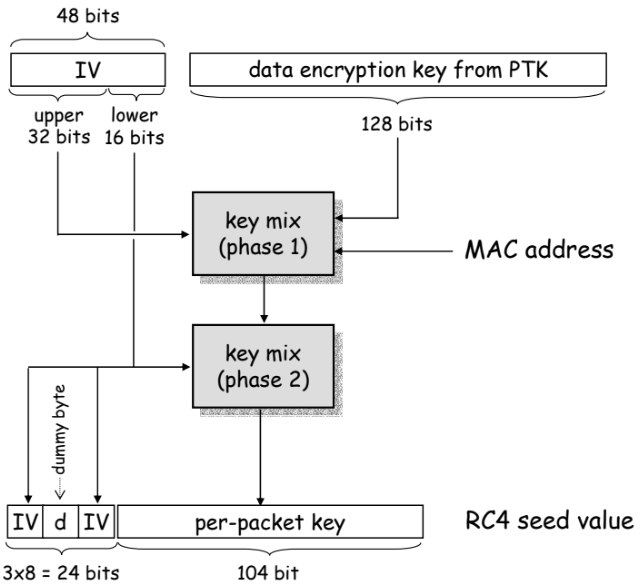
\includegraphics[width=0.8\linewidth]{tkip.png}
}

\frame{
	\frametitle{AES-CCMP}
	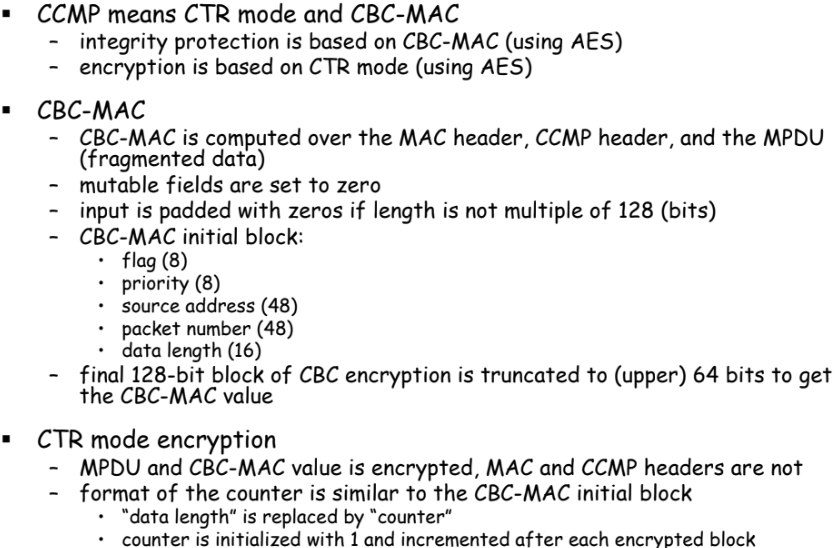
\includegraphics[width=0.8\linewidth]{ccmp.png}
}

\frame{
	\frametitle{EAP, EAPOL, RADIUS}
	\textbf{EAP (Extensible Authentication Protocol, Расширяемый Протокол Аутентификации)} — :
	\begin{enumerate}
	\item фреймворк аутентификации, который часто в беспроводных сетях и соединениях точка-точка;
	\item 4 типа сообщений:
	\begin{itemize}
		\item EAP reqiest - сообщение от клинета к серверу аунтефикации.
		\item EAP response - сообщение от сервера аунтефикации к клинету.
		\item EAP sucess
		\item EAP failure
	\end{itemize}
	\end{enumerate}

	\textbf{EAPOL (EAP over LAN)} — протокол для передачи ESP через LAN протолы.
	
	
}

	\frame {
	\begin{figure}
		%
\includegraphics[width=0.8\linewidth]{memes1.jpeg}
		
	\end{figure}
	}

\end{document}